\documentclass{article}

\usepackage[a4paper,hmargin=1.2in,vmargin=1.5in]{geometry}
\usepackage[parfill]{parskip} % for distance between paragraphs
\usepackage{ragged2e} % for alignment
\usepackage{hyperref} % for link
\usepackage{fancyhdr} % for header, footer
\usepackage{xcolor}  % for color
\usepackage{graphicx} % for figure
\usepackage{floatrow} % for formatting figures
\usepackage{enumitem} % for adjusting list spacing 
\usepackage{amsmath} 
\usepackage{amsthm} 
\usepackage{amssymb} 
\usepackage{esint}

\newtheorem{theorem}{Theorem}
\newtheorem{lemma}{Lemma}
\newtheorem{corollary}[theorem]{Corollary}
\newtheorem{proposition}{Proposition}[section]
\theoremstyle{remark}
\newtheorem*{remark}{Remark}

\setlength{\parskip}{0.5em}

\pagestyle{fancy}
\fancyhf{}
\lhead{190050113-190050080-190020010}
\rhead{CS 215}
\cfoot{Page \thepage}
\renewcommand{\footrulewidth}{1pt}

\usepackage{titlesec}
\titleformat{\section}
  {\Large\bfseries}{}{1em}{}

\title{Assignment 1: CS 215}

\author{
  \textbf{190050113} Shivam Raj
  \and
  \textbf{190050080} Pawan Kumar
  \and
  \textbf{190020010} Aman Singh
}

\date{\today}

\begin{document}

\pagenumbering{gobble}
\maketitle
\tableofcontents

\newpage
\pagenumbering{arabic}

\section{Question 1}
\textbf{(a)} The situation is equivalent to distributing $n$ books to $n$ people. The total number of ways of doing that is $n!$. There is only 1 way in which everyone gets his book back. So the probability of it happening is $\boxed{1/n!}$ \par

\textbf{(b)} There is only 1 way of distributing $m$ books to their respective $m$ owners. And for this way there are $(n-m)!$ ways of distributing the left $n-m$ books among left $n-m$ people for a total of $1\,\text{x}\,(n-m)!=(n-m)!$ ways. So the probability of it happening is $\boxed{(n-m)!/n!}$ \par

\textbf{(c)} There are $m!$ way of distributing the $m$ books belonging to the last $m$ people to the first $m$ people. And for each such way there are $(n-m)!$ ways of distributing the left $n-m$ books among left $n-m$ people for a total of $m!\,\text{x}\,(n-m)!=m!(n-m)!$ ways. So the probability of it happening is $\boxed{m!(n-m)!/n!}$ \par

\textbf{(d)} Every book has a probability $p$ of getting unclean which is independent of who picked up which book and independent of whether other books became unclean. So the probability of first $m$ people picking up books that are unclean will be $\prod_m p = \boxed{p^m}$ \par

\textbf{(e)} The probability of some \textit{particular} $m$ people picking up books that are unclean and the rest clean books is $p^m(1-p)^{n-m}$. But there are ${}^n C_m$ different ways of choosing a particular set of $m$ people from a group of $n$. So the probability of it happening is $\boxed{{}^n C_m p^m(1-p)^{n-m}}$\par
\section{Question 2}
\begin{center}
    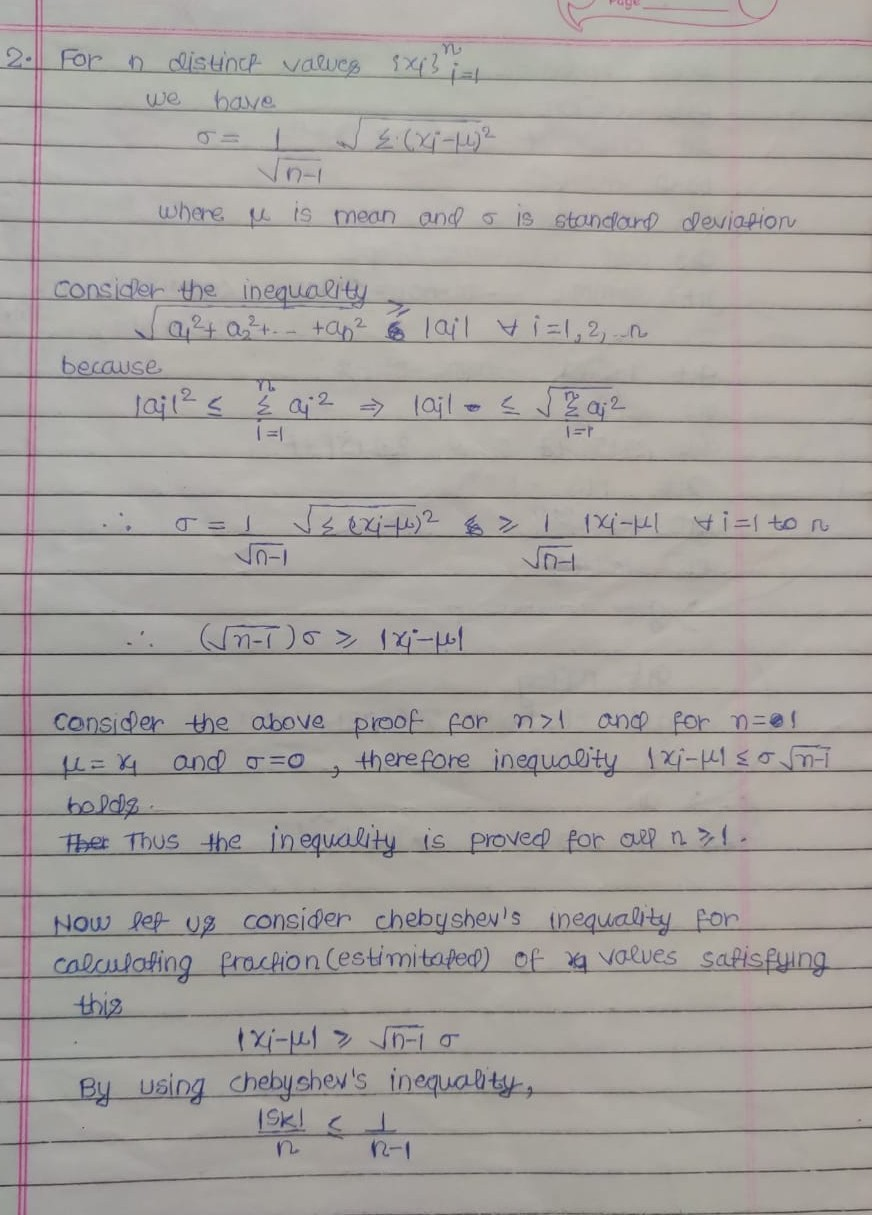
\includegraphics[width=\textwidth,height=\textheight,keepaspectratio]{q2_1.jpeg}
    \newpage
    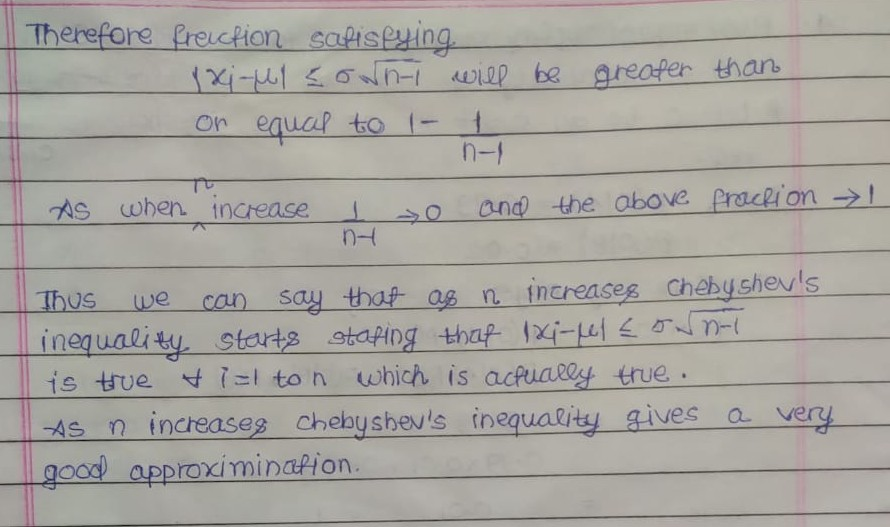
\includegraphics[width=\textwidth,height=\textheight,keepaspectratio]{q2_2.jpeg}
\end{center}

\section{Question 3}
\begin{center}
    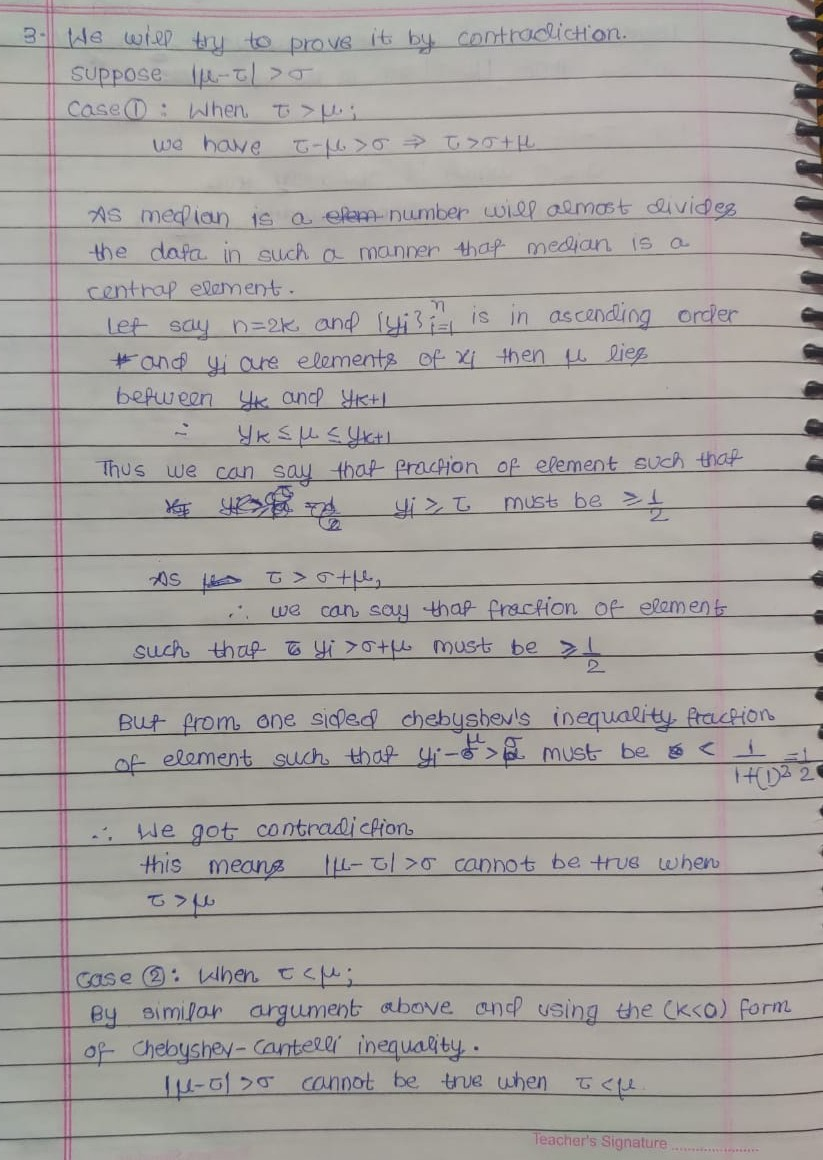
\includegraphics[width=\textwidth,height=\textheight,keepaspectratio]{q3_1.jpeg}
    \newpage
    
\includegraphics[width=\textwidth,height=\textheight,keepaspectratio]{q3_2.jpeg}
\end{center}
\section{Question 4}
\begin{center}
    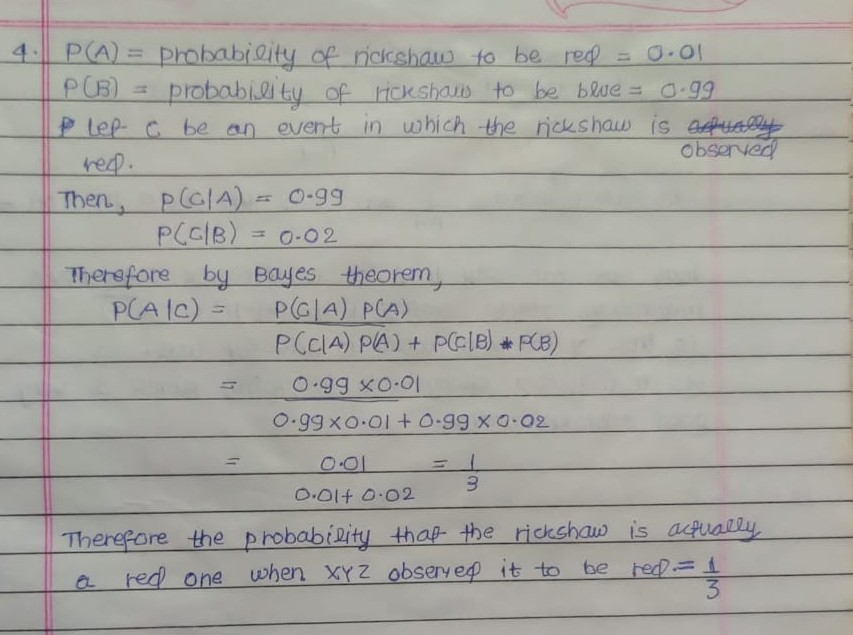
\includegraphics[width=\textwidth,height=\textheight,keepaspectratio]{q4_1.jpeg}
\end{center}
\newpage
\section{Question 5}
\hspace{2.5em} \textbf{(a)}.
\begin{center}
    \hspace{1.25em}$P(C_1|Z_1)= \frac{1}{3}$ \par
    \hspace{1.25em}$P(C_2|Z_1)=\frac{1}{3}$ \par
    \hspace{1.25em}$P(C_3|Z_1)=\frac{1}{3}$ \par
\end{center}

\hspace{2.5em} \textbf{(b)}
$P(H_3|C_1, Z_1)=\frac{1}{2}$ (if car is present behind first door so rest two doors have equal probability)\par
$P(H_3|C_2, Z_1)=1$ (if car is present behind door 2, so the host will always pick door 3) \par
$P(H_3|C_3, Z_1)=0$ (if  car is present behind door 3 , them host will never select it )\par


\hspace{2.5em} \textbf{(c)}
\begin {center}
$P(H_3|C_2, Z_1)=1 $ \par
$ P(C_2,Z_1)=P(C_2|Z_1) \times P(Z_1)=\frac{1}{3} \cdot \frac{1}{3}=\frac{1}{9}$\par
$ P(H_3|Z_1)= \frac{1}{3}\cdot\frac{1}{2}+\frac{1}{3}\cdot1+\frac{1}{3}\cdot0=\frac{1}{2} $ \par
\begin {align*}
P(H_3,Z_1) &= P(H_3|Z_1) \times P(Z_1) \\
&=\frac{1}{2} \cdot \frac{1}{3}\\
&= \frac{1}{6}
\end {align*}

\begin{align*}
    P(C_2|H_3,Z_1) & = \dfrac{P(H_3|C_2,Z_1)P(C_2,Z_1)}{P(H_3,Z_1)} \\
                   & = \dfrac{1 \times \frac{1}{9}}{\frac{1}{6}}    \\
                   & = \dfrac{2}{3}
\end{align*}


\end {center}

\hspace{2.5em} \textbf{(d)}
\begin{center}
    \begin{align*}
        P(C_1|H_3,Z_1) & = \dfrac{P(H_3|C_1,Z_1)P(C_1,Z_1)}{P(H_3,Z_1)}       \\
                       & =\dfrac{\frac{1}{2} \times \frac{1}{9}}{\frac{1}{6}} \\
                       & = \dfrac{1}{3}
    \end{align*}



\end{center}


\hspace{2.5em} \textbf{(e)}
$P(C_2|H_3,Z_1) > P(C_1|H_3,Z_1)$ \par
\hspace{3.0em}So, Switching will be beneficial \par

\hspace{2.5em} \textbf{(f)}
\begin{center}
    $ \forall_i P(H_3|C_i,Z_1)=\dfrac{1}{2}$ \par
    $\forall_i P(C_i,Z_1)=\dfrac{1}{3}$ \par

    $P(H_3|Z_1)=\dfrac{1}{2}$ \par
    $P(H_3,Z_1)=P(H_3|Z_1) \times P(Z_1)=\dfrac{1}{2} \cdot \dfrac{1}{3}=\dfrac{1}{6} $ \par
    \begin{align*}
        P(C_2|H_3,Z_1) & = \dfrac{P(H_3|C_2,Z_1)P(C_2,Z_1)}{P(H_3,Z_1)}        \\
                       & = \dfrac{\frac{1}{2} \times \frac{1}{9}}{\frac{1}{6}} \\
                       & = \dfrac{1}{3}
    \end{align*}
    \begin{align*}
        P(C_1|H_3,Z_1) & = \dfrac{P(H_3|C_1,Z_1)P(C_1,Z_1)}{P(H_3,Z_1)}       \\
                       & =\dfrac{\frac{1}{2} \times \frac{1}{9}}{\frac{1}{6}} \\
                       & = \dfrac{1}{3}
    \end{align*}

    \begin{align*}
        P(C_3|H_3,Z_1) & = \dfrac{P(H_3|C_3,Z_1)P(C_3,Z_1)}{P(H_3,Z_1)}       \\
                       & =\dfrac{\frac{1}{2} \times \frac{1}{9}}{\frac{1}{6}} \\
                       & = \dfrac{1}{3}
    \end{align*}

    $P(C_2|H_3,Z_1) = P(C_1|H_3,Z_1)$. So switching won't create any difference.



\end{center}





\newpage


% graph bohot faaltu hai

\section{Question 6}
The script for this question is under the file named \texttt{q6.m}.
Please note that the relative mean squared error values listed below are averaged from multiple runs of \texttt{q6.m} but the plots are representative of only one run.\
The relative mean squared error values in the case of 30\% and 60\% corruption are given below respectively :
\begin{description}[noitemsep]
    \item [Moving Median Filtering]\hspace{0.1em} 42.10
    \item [Moving Mean Filtering]\hspace{0.2em} 103.81
    \item [Moving Quartile Filtering]  0.01
\end{description}

\begin{center}
    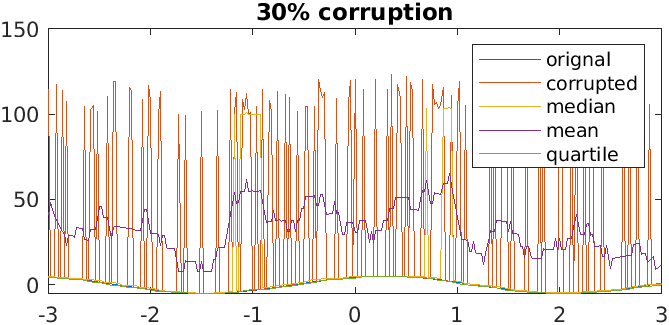
\includegraphics{q6(1).png}
\end{center}

\begin{description}[noitemsep]
    \item [Moving Median Filtering]\hspace{0.1em} 744.02
    \item [Moving Average Filtering]\hspace{0.2em} 376.55
    \item [Moving Quartile Filtering]  76.17
\end{description}

\begin{center}
    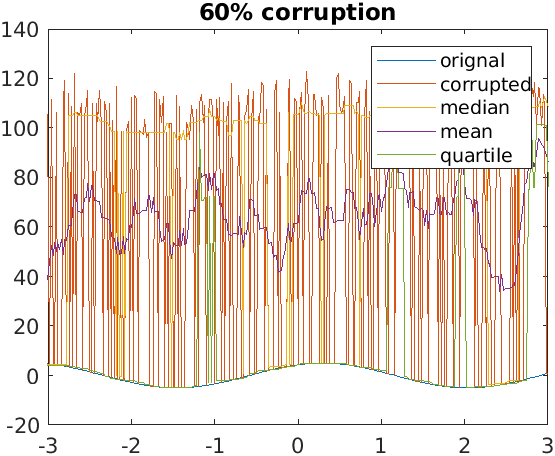
\includegraphics{q6(2).png}
\end{center}
In both the cases \textbf{moving quartile filtering} gives the least relative mean squared error. This can be explained as follows:\par
Lets choose a random $x$ point from the set $(\text{-}3:0.02:3)$. Let the set to be considered for filtering be $S = \{x_{\text{-}8}\,,x_{\text{-}7}\,\,...\,\, x_{0}\,\, ...\,\, x_{7},x_{8}\}$ where $x_0=x$ and $x_i>x_j$ for $i>j$. On an average if the probability of corruption is $p$ we can expect $p\,|S|$ values to be corrupted. All the corrupted values are necessarily greater than the uncorrupted ones. And as we consider $p$ values, here, to be $0.3$ or $0.6$ which is sufficiently greater than $0.75$ we can expect the 25th percentile to be in $S$ and hence close to $x$. \\
The average will be in between the the corrupted and uncorrupted (hence not close to $x$) and as the median is just the 50th percentile, chance of it being in $S$ is lower in the case of $p=0.3$ and much lower when $p=0.6$.

\newpage

\section{Question 7}
The script of this question is under the file named \texttt{q7.m} \par
\begin{align*}
    \mu      & = Old \; Mean                  \\
    \mu_n    & = New \; Mean                  \\
    \sigma   & = Old\; Standard \;Deviation   \\
    \sigma_n & = New \; Standard \; Deviation \\
    X        & = Old \;Median                 \\
    X_n      & = New\; Median                 \\
    A_i      & =Elemnts\; of \; array         \\
    b        & = New\;element                 \\
    n        & = Size \;of\; old\; array
\end{align*}

\begin{enumerate}
    \item
          \begin{align*}
              \sum_iA_i & =\mu\times n                    \\
              \mu_n     & =\dfrac{\sum_iA_i+b}{n+1}       \\
              \mu_n     & = \dfrac{(\mu \times n)+b}{n+1}
          \end{align*}

    \item \begin{itemize}
              \item \textbf{n is odd.} \par
                    if b is less than the element left to median then the new median will lie betwee old median and number left to it. \par
                    if b lies betwee number left and right to old median then new median will lie between old median and added number.\par
                    if b is greater than the number right to meadian the new median will lie between old median and number right to it.
              \item \textbf{n is even}\par
                    lets say the old median lies between i and j.\par
                    if $b < i$, $X_n=i$ \par
                    else if $ b > j, X_n=j$ \par
                    else $X_n=b$
          \end{itemize}
    \item \begin{align*}
              \sigma_n^2       & =\dfrac{\sum_i^n(A_i-\mu)^2 + (b-\mu)^2}{n}               \\
              n\cdot\sigma_n^2 & =\sum_i^n(A_i-\mu)^2 + (b-\mu)^2                          \\
              Now,                                                                         \\
              \sum_i^nA_i^2    & =(n-1)\sigma^2+2n\mu^2+-nx^2                              \\
              Using\; above \; result                                                      \\
              n\cdot\sigma^2_n & =(n-1)\sigma^2+n\mu^2+n\mu_n^2-2n\mu\mu_n+(b-\mu_n)^2     \\
                               & =(n-1)\sigma^2+b^2+n\mu^2+(n+1)\mu_n^2-2n\mu\mu_n-2b\mu_n \\
              Using\; result \; of \; first\; qsn                                          \\
              n\cdot\sigma_n^2 & =(n-1)\sigma^2+b^2+n\mu^2-(n+1)\mu_n^2                    \\
          \end{align*}
    \item We will increase the frequency of the bin which will contain the new element by 1.
\end{enumerate}

\end{document}
